\section{Introduction}
\label{sec:intro}

Masked diffusion language models (dLLMs) generate text by repeatedly resolving masked coordinates rather than committing tokens strictly from left to right~\citep{austin2021d3pm,hoogeboom2021argmax,campbell2022continuous,lou2024sedd,sahoo2024mdlm,nie2025smdm,nie2025llada,ye2025dream}. This parallel, iterative structure creates a quantization problem that is qualitatively different from perturbing a single feed-forward prediction. A small weight error can change a candidate token, reorder the global confidence frontier, alter which positions are committed, and redirect all subsequent states. Recent dLLM PTQ methods accordingly calibrate by mask state, denoising time, or decision frontier~\citep{lin2025qdllm,xu2025dllmquant,zhang2026quantdllm,yan2026starquant,huang2026faircalib}. What remains less clear is what output-law statement is licensed by local perturbation measurements.

\begin{figure}[t]
\centering
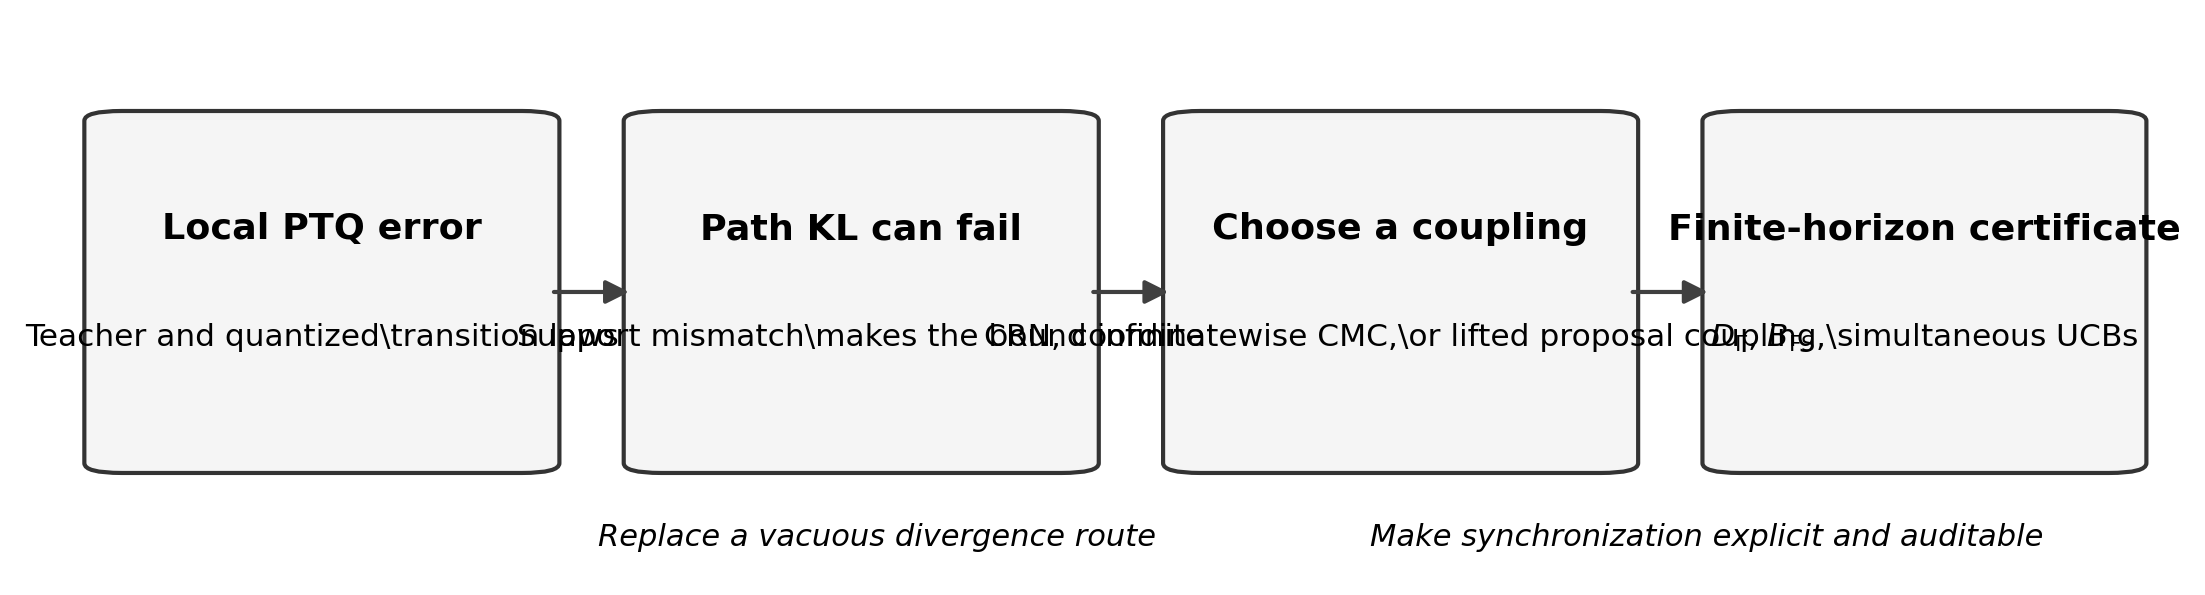
\includegraphics[width=.95\linewidth]{figures/figure_overview.png}
\caption{From local PTQ error to an output-law statement. A path-KL route can become infinite after support mismatch. Transport remains finite, but the result depends on the coupling used to synchronize the full-precision and quantized chains.}
\label{fig:overview}
\end{figure}

\paragraph{The obstruction.}
A conventional perturbation proof bounds KL divergence between full-precision (FP) and quantized trajectories and invokes data processing. For a masked decoder, however, a teacher-reachable transition may assign positive mass to a next state that the quantized transition assigns zero mass. The path KL is then infinite even when the terminal output laws are close. The divergence is a failure of the \emph{upper-bound route}, not evidence of catastrophic generation.

\paragraph{The coupling issue.}
We instead compare terminal laws with Wasserstein distance under normalized weighted Hamming. Any coupling $\Gamma$ of the two chains gives
\[
  \Wd(\mu_0^\star,\mu_0^q)
  \le D_\Gamma
  :=\Ex_\Gamma[d(X_0^\star,X_0^q)].
\]
The synchronization rule is therefore not a neutral implementation detail: it determines which valid upper bound is measured. This matters empirically. On the same W8 MDLM marginals, inverse-CDF common random numbers give terminal cost $0.9146$, whereas coordinatewise maximal coupling gives $0.2349$.

\paragraph{The masked-diffusion structure.}
The domain-specific idea is to stop at the first divergence. Under monotone copy-only generation, coordinates committed before the split cannot change again. Only the residual masked coordinates can contribute new terminal disagreement. This yields a diameter-safe bound whose two factors have distinct interpretations: bit width controls how often a split occurs, while the remaining reverse-time suffix controls how damaging that split can be.

\paragraph{Contributions.}
We make three claims.
\begin{enumerate}[leftmargin=1.6em,itemsep=2pt,topsep=2pt]
\item \textbf{Finite-horizon transport for irreversible masked generation.} We formalize the path-KL obstruction, derive teacher-prefix/quantized-suffix transport, and prove a first-divergence residual-mass bound together with finite-horizon and bounded-functional corollaries.
\item \textbf{Coupling-aware measurement.} For factorized transitions, coordinatewise maximal coupling exactly minimizes one-step weighted-Hamming cost. For non-factorized sample-then-select transitions, any proposal coupling can be pushed through the two deterministic, model-dependent selectors. We state explicitly what is one-step optimal and what is not.
\item \textbf{Statistical and empirical validation.} Simultaneous one-sided bounds cover both a fixed prompt suite and IID draws from a declared prompt population. Experiments isolate coupling, bit width, horizon, model, length, and sampler temperature. We also report preregistered negative investigations that fail to support stronger metric or calibration claims.
\end{enumerate}

\begin{table}[t]
\caption{Claims and evidence at a glance. Negative investigations narrow the interpretation rather than create additional contributions.}
\label{tab:claims}
\centering\small
\begin{tabular}{@{}p{.25\linewidth}p{.33\linewidth}p{.34\linewidth}@{}}
\toprule
Claim & Main evidence & Explicit boundary \\
\midrule
Path KL can be vacuous & support-mismatch proposition; deterministic selector examples & says nothing by itself about terminal task failure \\
First divergence controls worst-case damage & residual-mask theorem; early/middle/late damage $0.774/0.398/0.119$ & can be loose because splits may heal \\
Coupling changes the measured bound & W8 cost $0.915$ (CRN) vs. $0.235$ (CMC); official-sampler temperature panel & no universal coupling or path-optimality claim \\
Certificates extend beyond one suite & fixed-suite and prompt-population simultaneous UCBs; six-bit and second-model panels & exact-token metric; declared population only \\
Stronger metric/method claims are unsupported & additive-metric and calibration pilots & reported as negative investigations \\
\bottomrule
\end{tabular}
\end{table}

The intended contribution is therefore an analytical and measurement framework, not a new state-of-the-art quantizer. This positioning is deliberate: two follow-up attempts to turn the framework into a semantic metric and a transport-weighted calibration method did not pass their preregistered gates. Reporting those failures is part of the claim--evidence alignment of the paper.
